%!TEX root = ../../thesis.tex

\section{Quantitative Comparison of both Models}
\label{sec:Comparison}

\subsection{Prediction Accuracy}\label{sec:prediction_accuracy}
The high-dimensional physics-based model (Model B) is found to have a higher prediction accuracy compared to the low-dimensional data-driven model for the individual zones (Model A) presented in Section \ref{sec:Indiv_Zones}: According to Table \ref{tab:data_RMS_zones}, the mean RMS error for Model B across zones is $0.11^\circ \text{C}$ lower than for Model A. This is also illustrated in Figure \ref{fig:open_loop_trajectories}, which shows 7-day open-loop predictions of the temperature of a randomly selected holdout test week in the spring period, simulated with both models initialized with the measured temperature. The increase in RMS error from Model B to Model A is notably larger in the zones ``East'' (0.38) and ``Center'' (0.15), compared to the other zones (0.11, $-$0.03, 0.07, and 0.08). 

This provides new insight into the existing knowledge as we provide a quantitative comparison between the low-dimensional data-driven model and the high-dimensional physics-based model's prediction accuracy for the same multi-zone commercial building, which is in regular operation. The existing literature merely mentions that data-driven models are likely to have lower prediction accuracies than physics-based ones and, to the best of our knowledge, a quantitative comparison at this level is non-existent, as previous building models were developed for different testbeds, fictitious buildings or from simulated data.
%We show what prediction accuracies are achievable by each model when applied to a building subjected to disturbances such as occupancy, without using additional hardware such as occupancy sensors.

Next, we explore the extent to which this slightly lower prediction accuracy of Model A affects its resulting controller's closed-loop performance in a building energy efficiency example.

\begin{table}[hbtp]
\centering
\begin{tabular}{*8c}
\toprule
\multicolumn{8}{c}{Data-Driven Model} \\
\hline
Season & NW & W & S & E & NE & C & Mean \\ \hline
Fall & 0.98 & 0.61 & 0.28 & 0.42 & 0.28 & 0.36 & 0.488\\
Winter & 1.41 & 0.34 & 0.29 & 0.26 & 0.25 & 0.21 & 0.460\\
Spring & 0.56 & 0.25 & 0.31 & 0.71 & 0.17 & 0.34 & 0.390\\
\midrule
\midrule
\multicolumn{8}{c}{Physics-Based Model} \\
\hline
Season & NW & W & S & E & NE & C & Mean \\ \hline
Fall & 0.61 & 0.46 & 0.39 & 0.39 & 0.20 & 0.32 & 0.396\\
Winter & 0.55 & 0.39 & 0.34 & 0.32 & 0.18 & 0.24 & 0.338\\
Spring & 0.45 & 0.28 & 0.24 & 0.33 & 0.09 & 0.19 & 0.263\\
\bottomrule
\end{tabular}
\caption{RMS by Zone and Season for Data-Driven and Physics-Based Models}
\label{tab:data_RMS_zones}
\end{table}



\begin{figure}
\centering
\vspace*{-0.1cm}
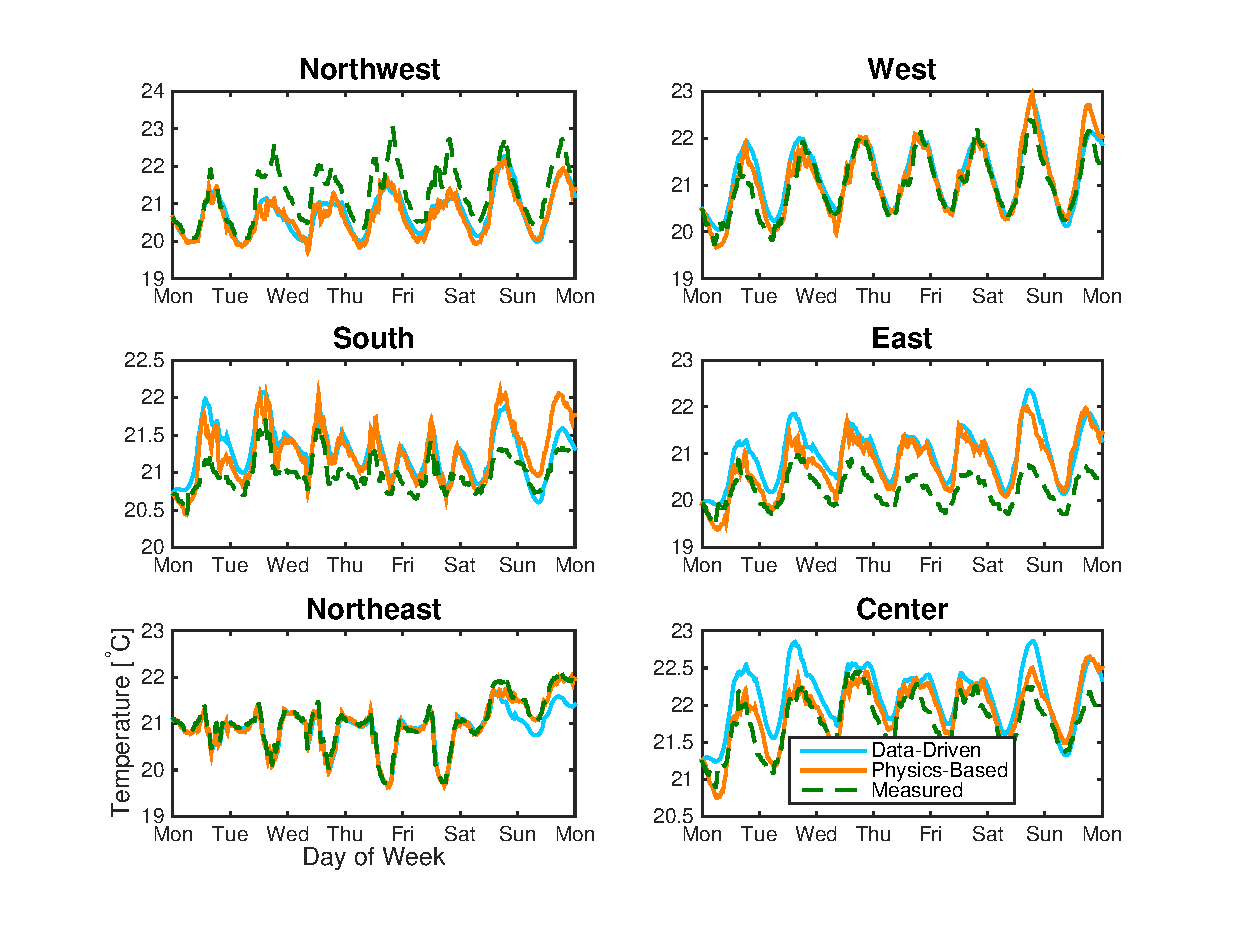
\includegraphics[width=\textwidth]{chapters/building_model/figures/open_loop_traj.eps}
\vspace*{-0.5cm}
\caption{Simulated Temperatures from the Data-Driven Model (blue), Physics-Based Model (orange) and Actual Temperatures (green) }
\vspace*{-0.5cm}
\label{fig:open_loop_trajectories}
\end{figure}
%The higher inaccuracy of the data-driven model becomes particularly apparent in zones Center and East, where the data-driven estimate notably deviates from the measured temperatures.

\subsection{Energy Efficient Control}\label{sec:energy_efficient_control}
In this section, we compare the performance of Model A and Model B for the purpose of energy efficiency. We formulate an MPC problem to find the optimal control strategy that minimizes the cost of HVAC operation over the same week used in Figure \ref{fig:open_loop_trajectories}, while guaranteeing the temperature to stay within a comfort zone $[T_{\text{min}}, T_{\text{max}}]$, which we chose as $[20^\circ \text{C}, 22^\circ \text{C}]$ \cite{Hansen:2013aa}, and confining the control input to the physical limits of the HVAC system $[u_{\text{min}}, u_{\text{max}}]$. This problem is formulated as follows:
\begin{equation}\label{eq:ee_controller}
\begin{split}
\min_{u, \varepsilon}~&\sum_{k=1}^N u(k)^2 + \rho \Vert\varepsilon\Vert_2 \\
\text{s.t.}~& x(0) = \bar{x}(0) \\
& x(k+1) = \begin{cases}
      \eqref{eq:temp_propagation_indiv}, & \text{Model A}  \\
      \eqref{eq:physics_model1}, & \text{Model B}
    \end{cases} \\
& u_{\text{min}}-\varepsilon \leq u(k) \leq u_{\text{max}}+\varepsilon\qquad \forall k\in[0, N-1]\\
& \begin{cases}
      T_{\text{min}} \leq x(k) \leq T_{\text{max}}, & \text{Model A}  \\
      T_{\text{min}} \leq Cx(k) \leq T_{\text{max}}, & \text{Model B}~\eqref{eq:physics_model_2}
    \end{cases}~ \forall k\in[1, N]
\end{split}
\end{equation}
The temperature is initialized with the measured temperature $\bar{x}(0)$ at the beginning of the week-long simulation. We use soft constraints on the control input with a penalty parameter $\rho$ to ensure the feasibility of the problem. The penalty represents the cost of increasing the airflow beyond the operating limits (temporary shutdown or overuse, both of which are harmful to the system). 
%The function $f(x(\cdot), u(\cdot), v(\cdot), q_{\text{IG}}(\cdot))$ is chosen to be either \eqref{eq:temp_propagation_indiv} for Model A or\eqref{eq:physics_model} for Model B.
To find the optimal control strategy, we make use of receding horizon control with a prediction horizon of three 15-minute time steps.


\begin{figure}
\centering
\vspace*{-0.4cm}
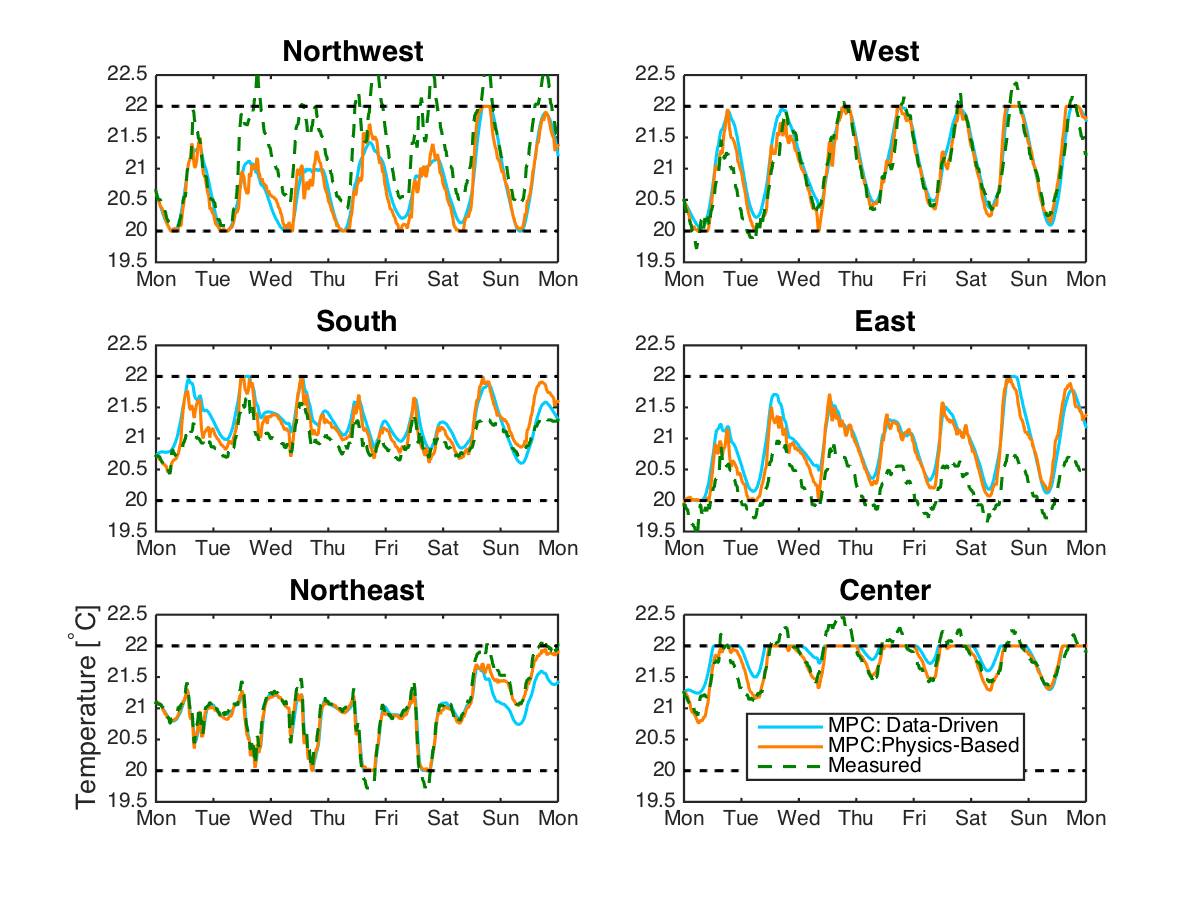
\includegraphics[width=\textwidth]{chapters/building_model/figures/Comparison_Temp.png}
\vspace*{-0.5cm}
\caption{Optimal Temperature for MPC with Data-Driven Model (blue), MPC with Physics-Based Model (orange) and Actual Temperature (green)}
\vspace*{-0.2cm}
\label{fig:MPC_comparison_temp}
\end{figure}

\begin{figure}
\centering
%\vspace*{-0.4cm}
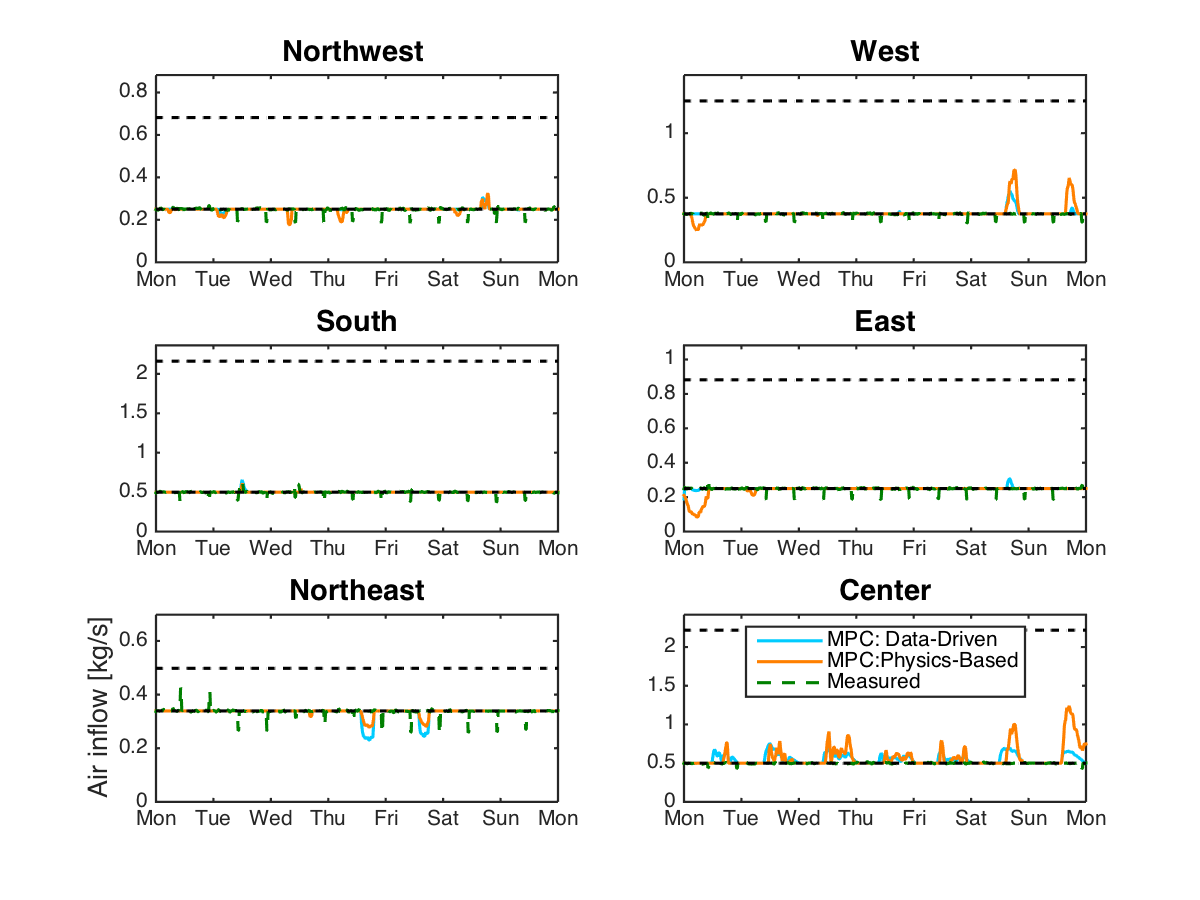
\includegraphics[width=\textwidth]{chapters/building_model/figures/Comparison_Flow.png}
\vspace*{-0.5cm}
\caption{Optimal Control Strategy for MPC with Data-Driven Model (blue), MPC with Physics-Based Model (orange) and Actual Input (green)}
%\vspace*{-0.2cm}
\label{fig:MPC_comparison_flow}
\end{figure}

Figure \ref{fig:MPC_comparison_temp} shows the temperature trajectory computed by the energy efficient controller \eqref{eq:ee_controller} computed with both models A and B, together with the measured temperature as a reference. 
It can be seen that both control schemes are capable of maintaining the temperature within $[20^\circ \text{C}, 22^\circ \text{C}]$, with a control strategy that is of comparable cost (1,006 and 1,731 for Model A and Model B, respectively, where $\rho=100$), shown in Figure \ref{fig:MPC_comparison_flow}. An interesting observation is that the largest difference in the control strategies is detected in zones ``East'' and ``Center'', which show a larger increase in RMS error from Model B to Model A.
%The dips of the computed control trajectory $u$ below the black dashed lines represent violations of the physical limits needed to maintain the temperature in the narrow range $[20^\circ, 22^\circ]$. 
Furthermore, it is interesting to observe that variations in the control input do not impact the periodicity of the temperature qualitatively, which can be explained by the regularity of the identified internal gains.

These findings suggest that both models perform equally well in designing an energy efficient control strategy. However, computing this strategy for Model A was cheap ($<5$ minutes) compared to Model B ($\approx 20$ hours) on a 2 GHz Intel Core i7, 16 GB 1600 MHz DDR3 machine. Further, we note that in real-world applications, the MPC would use state feedback to initialize the temperature with sensor measurements at every time step, whereas in our simulation, it operates in an ``open loop'' fashion and hence propagates the estimation error with time. This will reduce the difference in the prediction quality by both controllers even further, since the RMS error is now to be evaluated on a much shorter prediction horizon, thereby further corroborating the finding of almost identical control schemes.

Observing that Model A only suffers a negligible loss of accuracy compared to Model B for an open loop optimal control scheme, our findings suggest the applicability of Model A to other applications with temperature-critical zones in which even more precise temperature estimates are needed, e.g. long-term planning of reserve provision for frequency regulation.

%\textcolor{red}{While our findings suggest that Model A is suitable for tasks that can tolerate minor inaccuracies, such as energy efficient control, we note that for temperature-critical zones or applications in which precise temperature estimates are needed, e.g. long-term planning of reserve provision for frequency regulation, one might still want to choose the fine-level Model B for analysis.}



%%%%%%%%%%%%%%%%%%
%\subsection{Qualitative Comparison}
%We summarize the findings in the following:
%\begin{itemize}
%\item Model A is more \textit{amenable} to controller design due to its low dimensionality and hence considerably faster operation. This is of particular importance for \textit{scalability} considerations, since the computation time grows exponentially with the number of state variables, which renders Model B computationally intractable for online operation beyond a certain complexity. Indeed we observe that the computation for one step of \eqref{eq:ee_controller} exceeds 15 minutes $-$ the discretization time $-$ for a prediction horizon of five steps. Thus in frequency regulation, for instance, Model A's low dimensionality makes it suitable for reserve determination which must be computed for a time horizon of 24 hours.
%\item Identifying Model A with semiparametric regression only relies on temperature and VAV airflow data and the physical adjacency of zones, in contrast to Model B, which requires knowledge of the BRCM toolbox and a large amount of geometry and construction data of the buildings, many of which are often unknown \cite{Qie}. Hence, more effort is required to train the model on new buildings for Model B.
%\item The higher \textit{accuracy} of Model B proves useful for applications such as the control of temperature-critical zones and evaluation of controller performance through simulations, whereas Model A is preferably used for controller design and in applications where less emphasis is put on estimation errors, e.g. at night when building occupancy is low. 
%\item Model A assumes a uniform temperature among zones, which often encompass several rooms, whereas Model B can provide estimates for the temperature of individual rooms in a given zone. The number of parameters of Model A increases rapidly with the model complexity, which coupled with insufficient excitation of the system makes it hard to emulate the higher spatial \textit{granularity} with Model A. 
%\end{itemize}

%With a negligible contribution of $\mathbf{c}\cdot\mathbf{w}$ on the temperature evolution, equation \eqref{eq:Temperature_evolution} becomes
%\begin{equation}\label{eq:temp_evolution_decomp}
%x(n+1) = a x(n) + b u(n) + q_{\text{IG}}(n).
%\end{equation}
%As mentioned before, the main problem in the identification of the true physical value of $b$ lies in the lack of sufficient excitation of the temperature dynamics. Inspired by the prior knowledge of the VAV airflow, we chose $\hat{b}$ to be close to the approximated prior. For a fixed value of $\hat{b}$, the value of $\hat{a}$ minimizing the mean RMS is found to be $\approx 0.85$. Thus, fixing $a=0.85$, the only variable terms in \eqref{eq:temp_evolution_decomp} become $b u(n)$ and $q_{\text{IG}}$, and we thus obtain
%\begin{equation}
%\begin{aligned}
%0 &= \left(\hat{b}-b_{\text{opt}}\right)u(n) + \left(\hat{q}_{\text{IG}} - q_{\text{IG}}^{\text{opt}} \right)\\
%\hat{q}_{\text{IG}}(n) &= q_{\text{IG}}^{\text{opt}}(n) - \left(\hat{b}-b_{\text{opt}}\right)u(n)
%\end{aligned}
%\end{equation}
%by subtracting \eqref{eq:temp_evolution_decomp} for the optimal $b_{\text{opt}} = -0.03$ from \eqref{eq:temp_evolution_decomp} for the a-priori defined value $\hat{b} = -0.18$. We therefore find that different values of the estimated parameter $b$ result in a shift of the estimated internal gain. Further, we conclude that the internal gain estimated by the data-driven approach consists of two main contributions: the exogenous heating load due to occupancy and electric devices $q_{\text{exo}}$ (constant for a different season with weekly seasonality) and a variable term $q_{\text{bal}}$ that balances varying levels of the control input effect $|b\cdot u|$:
%\begin{equation}\label{eq:IG_decomposition}
%q_{\text{IG}}(n) = q_{\text{exo}}(n) + q_{\text{bal}}(n).
%\end{equation}
%Therefore the physically meaningful gain due to occupancy and electric devices $q_{\text{exo}}$ is masked and cannot be isolated from \eqref{eq:IG_decomposition}. It follows that different levels of internal gains for the different seasons (Figure \ref{fig:data_lump_qig} can only be assessed on a relative level
%
%In contrast to the data-driven approach, the physics-based model is able to isolate the exogenous occupancy load ...